\documentclass[aspectratio=169, 11pt]{beamer}

% =====================================================================
%  23CSE498 -- Project Phase 2 : Panel Review 1
%  Real-Time Adaptive Cross-Media Recommendation System
%  Type 3: Software Project
% =====================================================================

% --- Packages & Setup ---
\usepackage[utf8]{inputenc}
\usepackage[T1]{fontenc}
\usepackage{xcolor}
\usepackage{booktabs}
\usepackage{array}
\usepackage{amsmath}
\usepackage{amssymb}
\usepackage{graphicx}
\usepackage{tikz}
\usetikzlibrary{calc,positioning,arrows.meta,fit,backgrounds,shapes.geometric}

\graphicspath{{../}{./}}

% Try loading Open Sans; fallback if missing
\IfFileExists{opensans.sty}{\usepackage[default,scale=0.95]{opensans}}{}

% --- Branding Colors ---
\definecolor{amritaMaroon}{HTML}{A4123F}
\definecolor{amritaInk}{HTML}{1F2933}
\definecolor{amritaSlate}{HTML}{52616B}
\definecolor{amritaMist}{HTML}{F3F0F1}
\definecolor{amritaTeal}{HTML}{0F6F73}
\definecolor{amritaAmber}{HTML}{9C6000}

% --- Theme Setup ---
\usetheme{Madrid}
\usecolortheme[named=amritaMaroon]{structure}
\setbeamertemplate{navigation symbols}{}
\setbeamertemplate{footline}[frame number]
\setbeamertemplate{bibliography item}[text]
\setbeamertemplate{itemize items}[circle]
\setbeamercolor{itemize item}{fg=amritaMaroon}
\setbeamercolor{itemize subitem}{fg=amritaSlate}
\setbeamercolor{framesubtitle}{fg=amritaMist}
\setbeamerfont{framesubtitle}{size=\scriptsize}
\setbeamercolor{normal text}{fg=amritaInk}

% --- Status shorthands ---
\newcommand{\sOK}{\textcolor{amritaTeal}{\textbf{Functional}}}
\newcommand{\sINT}{\textcolor{amritaTeal}{\textbf{Integrated}}}
\newcommand{\sWIP}{\textcolor{amritaAmber}{\textbf{In progress}}}
\newcommand{\sPLN}{\textcolor{amritaSlate}{\textbf{Planned}}}

% --- EDIT THESE LINES ONLY -------------------------------------------
\newcommand{\teamnumber}{XX}
% Paste your Kaggle Step-4 LightGCN numbers here (Movies_and_TV):
\newcommand{\mvRecall}{0.0\underline{\hspace{4mm}}}
\newcommand{\mvNDCG}{0.0\underline{\hspace{4mm}}}
% ---------------------------------------------------------------------

\begin{document}

% =====================================================================
% TITLE SLIDE
% =====================================================================
\begin{frame}
    \begin{tikzpicture}[remember picture,overlay]
        \node[fill=amritaMaroon, text=white, font=\bfseries\footnotesize, anchor=north east, rounded corners=2pt, inner sep=5pt]
        at ($(current page.north east) + (-0.2cm,-0.2cm)$)
        {Type 3: Software Project};
    \end{tikzpicture}

    \centering
    \IfFileExists{logo.png}{
\includegraphics[width=2.6cm]{logo.png}\\[0.05cm]}{\vspace{0.2cm}}

    {\large \textbf{\textcolor{amritaMaroon}{Real-Time Adaptive Cross-Media Recommendation System}}} \\
    \vspace{0.04cm}
    {\scriptsize \textit{Unifying Movies, Books and Music with Semantic Embeddings,
     Knowledge-Graph Scoring and Graph Collaborative Learning}}\\
    \vspace{0.10cm}
    {\footnotesize \textbf{23CSE498 -- Project Phase 2 (Panel Review 1)} \quad | \quad \textbf{Team Number: \teamnumber}} \\
    \vspace{0.12cm}

    \begin{table}
        \centering
        \footnotesize
        \renewcommand{\arraystretch}{1.05}
        \begin{tabular}{|c|c|l|}
            \hline
            \textbf{S.No} & \textbf{Register Number} & \textbf{Student Name} \\
            \hline
            1 & CB.SC.U4CSE23051 & Sanjay A. K. \\
            \hline
            2 & CB.SC.U4CSE23022 & Eswara Raj M. \\
            \hline
            3 & CB.SC.U4CSE23324 & Aditya Vijay \\
            \hline
            4 & CB.SC.U4CSE23359 & Himaneesh Reddy Jangalapalli \\
            \hline
        \end{tabular}
    \end{table}
    \vspace{0.06cm}

    {\footnotesize Guides: \textbf{Dr.~Bagavathi Sivakumar P.} \ \& \ \textbf{Dr.~Krishna Priya G.},
     Department of CSE} \\
    \vspace{0.06cm}
    {\scriptsize Amrita School of Computing, Coimbatore \quad|\quad \today}
\end{frame}

% =====================================================================
% SECTION 1 -- ARCHITECTURE (Rubric: 5 Marks)
% =====================================================================
\section{Architecture \& Module Design}

\begin{frame}{1. Software Architecture \& Module Design}
\framesubtitle{Rubric: Architecture Diagram, Module Interaction, APIs, DB Schema \& Deployment (5 Marks)}
\vspace{-1.5mm}
\begin{center}
\begin{tikzpicture}[
  scale=0.80, transform shape, font=\scriptsize,
  strip/.style={fill=amritaMaroon, draw=amritaMaroon, rounded corners=1.5pt},
  band/.style={rounded corners=3pt, draw=amritaMaroon!25, fill=amritaMaroon!5},
  sband/.style={rounded corners=3pt, draw=amritaAmber!35, fill=amritaAmber!5},
  astrip/.style={fill=amritaAmber, draw=amritaAmber, rounded corners=1.5pt},
  box/.style={rounded corners=2pt, draw=amritaMaroon!60, fill=white, align=center,
              minimum height=8mm, inner xsep=3pt, font=\scriptsize},
  store/.style={rounded corners=2pt, draw=amritaTeal!70, fill=amritaTeal!8, align=center,
              minimum height=9mm, inner xsep=3pt, font=\scriptsize},
  offb/.style={rounded corners=2pt, draw=amritaAmber!75, fill=white, align=center,
              minimum height=9.5mm, minimum width=3.2cm, inner xsep=2pt, font=\tiny},
  cap/.style={font=\tiny\itshape, text=amritaSlate, anchor=west},
  flow/.style={-{Latex[length=2.2mm]}, draw=amritaMaroon, line width=0.55pt},
  bidi/.style={{Latex[length=2.2mm]}-{Latex[length=2.2mm]}, draw=amritaTeal, line width=0.55pt},
  train/.style={-{Latex[length=2.2mm]}, draw=amritaAmber, line width=0.55pt, dashed},
  lbl/.style={font=\tiny\itshape, text=amritaSlate}
]

% ---------------- BAND A : CLIENT ----------------
\draw[band]  (0.62,6.20) rectangle (10.60,7.60);
\draw[strip] (0.00,6.20) rectangle (0.56,7.60);
\node[white, font=\tiny\bfseries, rotate=90] at (0.28,6.90) {CLIENT};
\node[cap] at (0.75,7.44) {React 19 $\cdot$ Vite $\cdot$ TailwindCSS $\cdot$ Framer Motion $\cdot$ axios \ \ (14 components, 2 routed pages)};
\node[box, minimum width=2.15cm] (uiA) at (1.80,6.80) {Search bar +\\autocomplete};
\node[box, minimum width=2.15cm] (uiB) at (4.20,6.80) {Result cards +\\score bars};
\node[box, minimum width=2.15cm] (uiC) at (6.60,6.80) {Like / bookmark /\\skip / rate};
\node[box, minimum width=2.15cm] (uiD) at (9.00,6.80) {Profile selector +\\detail modal};

% ---------------- BAND B : API ----------------
\draw[band]  (0.62,4.75) rectangle (10.60,6.00);
\draw[strip] (0.00,4.75) rectangle (0.56,6.00);
\node[white, font=\tiny\bfseries, rotate=90] at (0.28,5.37) {API};
\node[cap] at (0.75,5.86) {FastAPI $\cdot$ Pydantic v2 schemas $\cdot$ CORS middleware $\cdot$ lifespan singletons $\cdot$ OpenAPI \texttt{/docs}};
\node[box, minimum width=9.40cm, minimum height=9mm, font=\tiny\ttfamily] (api) at (5.61,5.24)
  {POST /recommend \ \ POST /recommend/item \ \ POST /interactions\\
   GET /search/suggest \ \ GET /interactions/\{user\}/\{item\} \ \ GET /health};

% ---------------- BAND C : ENGINE ----------------
\draw[band]  (0.62,2.40) rectangle (10.60,4.45);
\draw[strip] (0.00,2.40) rectangle (0.56,4.45);
\node[white, font=\tiny\bfseries, rotate=90] at (0.28,3.42) {ENGINE};
\node[cap] at (0.75,4.33) {Request-time recommendation pipeline (candidate generation $\rightarrow$ multi-signal rerank)};
\node[box, minimum width=3.00cm] (cre) at (2.30,3.82) {Creator / person match\\\tiny exact $\rightarrow$ prefix $\rightarrow$ substring};
\node[box, minimum width=3.10cm] (sbe) at (5.85,3.82) {Sentence-BERT encoder\\\tiny all-MiniLM-L6-v2 $\rightarrow$ 384-d};
\node[box, minimum width=2.50cm] (ann) at (9.15,3.82) {Qdrant ANN\\\tiny cosine, top-$N$};
\draw[flow] (sbe) -- (ann);

\node[box, minimum width=2.20cm] (sig1) at (1.95,2.86) {EMA session\\$\lambda_e = 0.15$};
\node[box, minimum width=2.20cm] (sig2) at (4.35,2.86) {LightGCN\\$\lambda_g = 0.20$};
\node[box, minimum width=2.20cm] (sig3) at (6.75,2.86) {KG proximity\\$\lambda_k = 0.08$};
\node[box, minimum width=2.20cm] (sig4) at (9.15,2.86) {Profile fit\\$\lambda_p = 0.10$};

% ---------------- BAND D : DATA ----------------
\draw[band]  (0.62,0.95) rectangle (10.60,2.15);
\draw[strip] (0.00,0.95) rectangle (0.56,2.15);
\node[white, font=\tiny\bfseries, rotate=90] at (0.28,1.55) {DATA};
\node[cap] at (0.75,2.03) {Persistence layer and exported model artifacts};
\node[store, minimum width=3.00cm] (qd) at (2.55,1.48) {Qdrant \texttt{content}\\\tiny 48{,}294 $\times$ 384 vectors, HNSW};
\node[store, minimum width=3.40cm] (my) at (6.10,1.48) {MySQL \texttt{cross\_media\_recs}\\\tiny content\_entities $\cdot$ user\_profiles $\cdot$ user\_interactions};
\node[store, minimum width=2.35cm] (ar) at (9.35,1.48) {Artifact store\\\tiny lightgcn\_embeddings.npz};

% ---------------- SIDEBAR : OFFLINE ----------------
\draw[sband]  (11.05,0.95) rectangle (15.10,7.60);
\draw[astrip] (11.05,0.95) rectangle (11.61,7.60);
\node[white, font=\tiny\bfseries, rotate=90] at (11.33,4.28) {OFFLINE / TRAINING PIPELINE};
\node[offb] (o1) at (13.40,6.85) {\textbf{Raw datasets}\\TMDb 5000 $\cdot$ Google Books $\cdot$ Spotify Songs};
\node[offb] (o2) at (13.40,5.65) {\texttt{preprocessing.}\\\texttt{build\_content\_catalog}\\unified 14-column schema};
\node[offb] (o3) at (13.40,4.45) {\texttt{embeddings.}\\\texttt{build\_embeddings}\\SHA-256 cache, 384-d};
\node[offb] (o4) at (13.40,3.25) {\texttt{embeddings.}\\\texttt{build\_qdrant\_collection}\\vector + payload upsert};
\node[offb] (o5) at (13.40,1.90) {\texttt{models.graph.}\\\texttt{train\_lightgcn}\\BPR loss, 3 layers, $d{=}64$};
\draw[train] (o1) -- (o2);
\draw[train] (o2) -- (o3);
\draw[train] (o3) -- (o4);
\draw[train] (o4) -- (o5);

% ---------------- INTER-BAND FLOWS ----------------
\draw[flow] (5.61,6.20) -- (5.61,6.00);
\node[lbl, anchor=west] at (5.72,6.10) {HTTPS / JSON};
\draw[flow] (5.61,4.75) -- (5.61,4.45);
\node[lbl, anchor=west] at (5.72,4.60) {validated request $(q,\,u,\,K,\,type)$};
\draw[bidi] (5.61,2.40) -- (5.61,2.15);
\node[lbl, anchor=west] at (5.72,2.27) {vector search $\cdot$ event log $\cdot$ embedding load};

% dashed training-time write path
\draw[train] (13.40,1.425) -- (13.40,0.60) -- (8.00,0.60) -- (8.00,0.95);
\node[lbl, anchor=west, text=amritaAmber] at (8.15,0.60) {training-time artifact writes};
\end{tikzpicture}
\end{center}
\vspace{-2mm}
{\scriptsize \textbf{Hybrid ranking contract:}\;
$S(i,u,q)=S_{\mathit{sem}}(i,q)+\lambda_g S_{\mathit{graph}}(i,u)+\lambda_e S_{\mathit{ema}}(i,u)+\lambda_k S_{\mathit{kg}}(i,q)+\lambda_p S_{\mathit{profile}}(i,u)$
\; -- every sub-score is returned to the UI, so each ranking is explainable.}
\end{frame}

% ---------------------------------------------------------------------
\begin{frame}[fragile]{1. Module Decomposition, API Contracts \& Database Schema}
\framesubtitle{Modular breakdown $\cdot$ REST contract $\cdot$ relational schema $\cdot$ deployment topology}
\vspace{-1mm}
\begin{columns}[T]
\column{0.52\textwidth}
{\scriptsize \textbf{Module breakdown and ownership}}
\vspace{-1mm}
\begin{table}
\centering
\tiny
\renewcommand{\arraystretch}{1.18}
\begin{tabular}{p{1.70cm} p{2.35cm} p{2.35cm}}
\toprule
\textbf{Module} & \textbf{Responsibility} & \textbf{Implementation} \\
\midrule
Data layer & Schema mapping $\phi_d$, cleaning, catalog build & \texttt{preprocessing/} \\
Embedding layer & SBERT encode, hash-cache, Qdrant upsert & \texttt{embeddings/} \\
Retrieval & ANN search, creator match, filters & \texttt{qdrant\_recommender.py} \\
Adaptation & EMA profile vector update / score & \texttt{ema\_recommender.py} \\
Graph CF & LightGCN train, export, rerank & \texttt{models/graph/} \\
Knowledge graph & Entity + profile scoring, rerank & \texttt{knowledge\_graph.py} \\
Persistence & Catalog, profiles, interactions, EMA blobs & \texttt{mysql\_store.py} \\
API gateway & Validation, DI, error mapping, CORS & \texttt{app.py}, \texttt{schemas.py} \\
Presentation & Search, cards, signals, feedback & \texttt{frontend/src/} \\
\bottomrule
\end{tabular}
\end{table}

\column{0.455\textwidth}
{\scriptsize \textbf{Representative API contract}}
\vspace{-1mm}
{\tiny
\begin{verbatim}
POST /recommend
{ "query":"space adventure with aliens",
  "user_id":"user_scifi", "top_k":5,
  "content_type": null }
--> { "results":[ { "global_id","title",
     "content_type","creators","categories",
     "score","semantic_score","graph_score",
     "ema_score","kg_score","profile_score" } ] }
\end{verbatim}
}
\vspace{-3mm}
{\scriptsize \textbf{Relational schema (MySQL 8)}}
\begin{itemize}\tiny
  \item \texttt{content\_entities}(\underline{global\_id}, content\_type, source, source\_id, title, description, creators, categories, release\_date, popularity, rating, text\_hash)
        --- \textit{idx:} \texttt{content\_type}, \texttt{source}
  \item \texttt{user\_profiles}(\underline{user\_id}, age\_group, profession, interests, \texttt{ema\_vector})
  \item \texttt{user\_interactions}(\underline{id}, user\_id, entity\_id $\rightarrow$ FK, event\_type, event\_value, timestamp)
        --- \textit{idx:} \texttt{(user\_id, timestamp)}, \texttt{entity\_id}
\end{itemize}
\vspace{-1mm}
{\scriptsize \textbf{Deployment topology}}
\begin{itemize}\tiny
  \item Qdrant via Docker (\texttt{6333/6334}); MySQL 8; Uvicorn ASGI workers; Vite static build served same-origin.
  \item GPU training decoupled to Kaggle T4 --- only the \texttt{.npz} ships back, so the served API needs no GPU.
  \item 12-factor config via \texttt{.env} / \texttt{settings.py}; \sPLN\ Docker Compose + GitHub Actions CI.
\end{itemize}
\end{columns}
\end{frame}

% =====================================================================
% SECTION 2 -- IMPLEMENTATION PROGRESS (Rubric: 8 Marks)
% =====================================================================
\section{Implementation Progress}

\begin{frame}{2. Implementation Progress ($\approx$60\%) \& Module Functionality}
\framesubtitle{Rubric: Backend, Frontend, Database \& Core Modules Functional (8 Marks)}
\vspace{-2mm}
\begin{table}
    \centering
    \tiny
    \renewcommand{\arraystretch}{1.06}
    \begin{tabular}{p{1.95cm} p{6.75cm} p{1.45cm} c}
        \toprule
        \textbf{Subsystem} & \textbf{Current implementation state (verified)} & \textbf{Evidence} & \textbf{Status} \\
        \midrule
        Data pipeline & 3 sources normalised into one 14-column catalog: \textbf{48{,}294} items (28{,}352 music / 15{,}139 books / 4{,}803 movies) & \texttt{content\_catalog.csv} & \sOK \\
        Embeddings & SBERT \texttt{all-MiniLM-L6-v2}, \textbf{48{,}294 $\times$ 384} float32; SHA-256 hash skips unchanged rows on rebuild & \texttt{content\_embeddings.npy} & \sOK \\
        Vector search & Qdrant collection with full payloads; cosine ANN plus optional \texttt{content\_type} filter inside the search & \texttt{/recommend} 200 OK & \sOK \\
        Creator search & Deterministic exact / prefix / substring match over \texttt{creators}, plus a typeahead endpoint & \texttt{/search/suggest} & \sOK \\
        Database layer & MySQL 8: 3 tables, FK + 4 indices, idempotent upserts, auto-migration script & \texttt{scripts/init\_mysql.py} & \sINT \\
        Adaptation (EMA) & User vector in the same 384-d space, updated synchronously on every event ($\alpha{=}0.25$) & \texttt{ema\_score} in payload & \sOK \\
        Graph CF & PyTorch LightGCN, BPR loss, $d{=}64$, $L{=}3$; artifact exported and consumed by the reranker & \texttt{lightgcn\_...npz} & \sOK \\
        Knowledge graph & \textbf{564 nodes / 845 edges} (233 creator, 125 music, 74 genre, 68 book, 58 movie, 6 user) + interactive visualizer & \texttt{kg\_visualizer.html} & \sOK \\
        Backend APIs & \textbf{7} FastAPI endpoints, Pydantic v2 validation, typed error mapping (400 / 503), OpenAPI docs & \texttt{/docs} & \sOK \\
        Frontend UI & React 19 SPA: 14 components, 2 routed pages, filters, score bars, similar-item drawer, feedback & \texttt{npm run build} & \sOK \\
        Integration & Loop closed: UI feedback $\rightarrow$ MySQL $\rightarrow$ EMA update $\rightarrow$ ranking shifts, with no retraining & live demo & \sINT \\
        Quality gate & \textbf{55 / 55} unit + integration tests green in \textbf{7.81 s} across 5 suites & \texttt{pytest -q} & \sOK \\
        \midrule
        Benchmark eval & Amazon Reviews 2023 pipeline + GPU notebook ready; \textbf{Movies\_and\_TV} trained, Books / CDs queued & Kaggle T4 & \sWIP \\
        Remaining 40\% & Neo4j migration, Docker Compose + CI/CD, P95 latency benchmarking, diversity rerank, user study & Review 2 & \sPLN \\
        \bottomrule
    \end{tabular}
\end{table}
\vspace{-1mm}
{\scriptsize \textbf{Demonstration evidence:} live UI walkthrough $\cdot$ Swagger \texttt{/docs} request--response $\cdot$ \texttt{pytest} run $\cdot$
interactive KG visualizer $\cdot$ \textbf{25} commits on \texttt{main}.}
\end{frame}

% ---------------------------------------------------------------------
\begin{frame}{2. Model Design -- Multi-Signal Ranking Pipeline}
\framesubtitle{How one query becomes an explainable ranked list spanning three media domains}
\vspace{-2mm}
\begin{center}
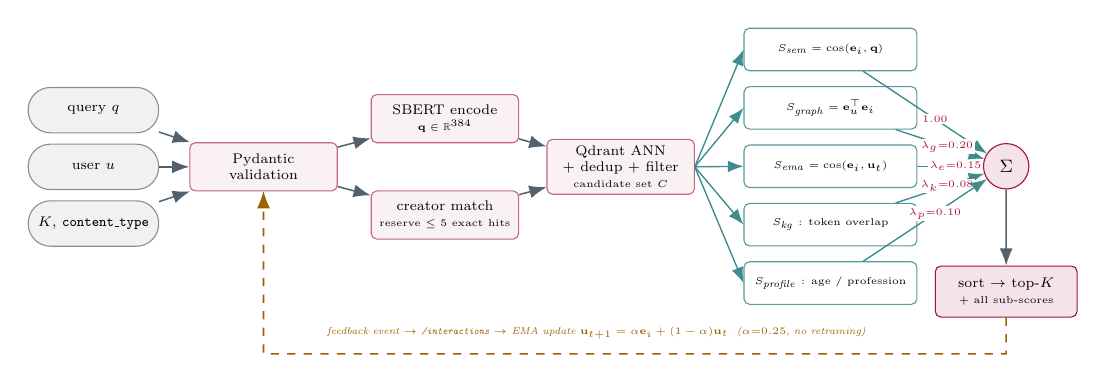
\begin{tikzpicture}[
  scale=0.72, transform shape, font=\scriptsize,
  inp/.style={rounded corners=8pt, draw=amritaSlate!70, fill=amritaMist, align=center,
              minimum height=8mm, minimum width=2.3cm, font=\scriptsize},
  proc/.style={rounded corners=2pt, draw=amritaMaroon!65, fill=amritaMaroon!6, align=center,
              minimum height=8.5mm, minimum width=2.6cm, font=\scriptsize},
  head/.style={rounded corners=2pt, draw=amritaTeal!70, fill=white, align=center,
              minimum height=7.5mm, minimum width=3.05cm, font=\tiny},
  sum/.style={circle, draw=amritaMaroon, fill=amritaMaroon!12, minimum size=8mm, font=\small},
  outp/.style={rounded corners=2pt, draw=amritaMaroon, fill=amritaMaroon!12, align=center,
              minimum height=9mm, minimum width=2.5cm, font=\scriptsize},
  fl/.style={-{Latex[length=2.2mm]}, draw=amritaSlate, line width=0.55pt},
  fw/.style={-{Latex[length=2mm]}, draw=amritaTeal!80, line width=0.5pt},
  wt/.style={font=\tiny, text=amritaMaroon, fill=white, inner sep=1pt}
]
% ---- inputs
\node[inp] (q)  at (0,4.55) {query $q$};
\node[inp] (u)  at (0,3.55) {user $u$};
\node[inp] (kk) at (0,2.55) {$K$, \texttt{content\_type}};

% ---- validation
\node[proc] (val) at (3.00,3.55) {Pydantic\\validation};
\draw[fl] (q)  -- (val);
\draw[fl] (u)  -- (val);
\draw[fl] (kk) -- (val);

% ---- candidate generation
\node[proc] (enc) at (6.20,4.40) {SBERT encode\\\tiny $\mathbf{q}\in\mathbb{R}^{384}$};
\node[proc] (cre) at (6.20,2.70) {creator match\\\tiny reserve $\leq 5$ exact hits};
\draw[fl] (val) -- (enc);
\draw[fl] (val) -- (cre);
\node[proc] (cand) at (9.30,3.55) {Qdrant ANN\\+ dedup + filter\\\tiny candidate set $C$};
\draw[fl] (enc)  -- (cand);
\draw[fl] (cre)  -- (cand);

% ---- scoring heads
\node[head] (h1) at (13.00,5.62) {$S_{\mathit{sem}}=\cos(\mathbf{e}_i,\mathbf{q})$};
\node[head] (h2) at (13.00,4.59) {$S_{\mathit{graph}}=\mathbf{e}_u^{\top}\mathbf{e}_i$};
\node[head] (h3) at (13.00,3.56) {$S_{\mathit{ema}}=\cos(\mathbf{e}_i,\mathbf{u}_t)$};
\node[head] (h4) at (13.00,2.53) {$S_{\mathit{kg}}$ : token overlap};
\node[head] (h5) at (13.00,1.50) {$S_{\mathit{profile}}$ : age / profession};
\foreach \h in {h1,h2,h3,h4,h5}{\draw[fw] (cand.east) -- (\h.west);}

% ---- blend
\node[sum] (sig) at (16.10,3.56) {$\Sigma$};
\draw[fw] (h1) -- (sig) node[wt, pos=0.58] {$1.00$};
\draw[fw] (h2) -- (sig) node[wt, pos=0.58] {$\lambda_g{=}0.20$};
\draw[fw] (h3) -- (sig) node[wt, pos=0.58] {$\lambda_e{=}0.15$};
\draw[fw] (h4) -- (sig) node[wt, pos=0.58] {$\lambda_k{=}0.08$};
\draw[fw] (h5) -- (sig) node[wt, pos=0.58] {$\lambda_p{=}0.10$};

\node[outp] (out) at (16.10,1.35) {sort $\rightarrow$ top-$K$\\\tiny + all sub-scores};
\draw[fl] (sig) -- (out);

% ---- feedback loop
\draw[fl, dashed, draw=amritaAmber]
  (out.south) -- (16.10,0.25) -- (3.00,0.25) -- (3.00,3.125);
\node[font=\tiny\itshape, text=amritaAmber, anchor=west] at (4.00,0.62)
  {feedback event $\rightarrow$ \texttt{/interactions} $\rightarrow$ EMA update
   $\mathbf{u}_{t+1}=\alpha\mathbf{e}_i+(1-\alpha)\mathbf{u}_t$ \ ($\alpha{=}0.25$, no retraining)};
\end{tikzpicture}
\end{center}
\vspace{-2mm}
\begin{columns}[T]
\column{0.49\textwidth}
{\scriptsize \textbf{Why each head exists}}
\begin{itemize}\tiny
  \item \textbf{Semantic} --- solves cold start; the only head defined for an item with zero interactions.
  \item \textbf{LightGCN} --- captures collaborative behaviour text cannot express; used as a reranker, never as the candidate generator.
  \item \textbf{EMA} --- reacts within a single click: graph retraining takes hours, an EMA update is one vector write.
\end{itemize}
\column{0.49\textwidth}
{\scriptsize \textbf{LightGCN configuration (as trained)}}
\begin{itemize}\tiny
  \item Propagation $\mathbf{e}^{(\ell)}_u=\sum_{i\in\mathcal{N}_u}\mathbf{e}^{(\ell-1)}_i/\sqrt{|\mathcal{N}_u||\mathcal{N}_i|}$ with layer-mean readout.
  \item BPR pairwise loss $-\sum\ln\sigma(\hat y_{ui}-\hat y_{uj})+\lambda\lVert\Theta\rVert^2$ --- implicit, positive-only feedback.
  \item $d{=}64$, $L{=}3$, lr $10^{-3}$, weight decay $10^{-4}$, batch 1024, seed 42.
\end{itemize}
\end{columns}
\end{frame}

% ---------------------------------------------------------------------
\begin{frame}{2. Knowledge Graph -- Structure, Scoring and Cross-Media Role}
\framesubtitle{The component that actually makes the system \emph{cross}-media}
\vspace{-1mm}
\begin{columns}[T]
\column{0.45\textwidth}
{\scriptsize \textbf{Built graph (from the live catalog)}}
\begin{itemize}\tiny
  \item \textbf{564 nodes / 845 edges}: 233 \emph{Creator}, 125 \emph{Song}, 74 \emph{Genre}, 68 \emph{Book}, 58 \emph{Movie}, 6 \emph{User}.
  \item Edges: \texttt{HAS\_GENRE} (498), \texttt{CREATED\_BY} (319), \texttt{AFFINITY} (10), \texttt{RECOMMENDED} (LightGCN-weighted).
  \item \emph{Profession}, \emph{Age Group} and \emph{Interest} nodes come from declared, consent-based profile fields --- no scraping.
\end{itemize}
\vspace{0.5mm}
{\scriptsize \textbf{Technical role in the pipeline}}
\begin{itemize}\tiny
  \item \textbf{Cross-domain bridge.} Creator / genre / profile namespaces are \emph{shared}, so a path can leave a \emph{Movie} and reach a \emph{Book} with no domain-specific edge.
  \item \textbf{Cold-start rescue.} KG and profile scores are defined for items with \emph{zero} interactions --- exactly where $S_{\mathit{graph}}$ is undefined.
  \item \textbf{Safety.} A negative weight $w_-\!=\!0.25$ demotes categories flagged unsuitable for an age group (horror / crime for \texttt{family}, \texttt{teen}).
  \item \textbf{Explainability.} \texttt{kg\_score} and \texttt{profile\_score} are returned per item and drawn as bars in the UI.
\end{itemize}
\vspace{0.5mm}
{\tiny
$P(u,i)=\{u\!\rightarrow\!e_1\!\rightarrow\!\cdots\!\rightarrow\!i\}$, \ $e_k\in\mathcal{E}_{creator}\cup\mathcal{E}_{genre}\cup\mathcal{E}_{profile}$
\\[1mm]
$S_{\mathit{kg}}(i,q)=\min\!\Big(1,\dfrac{|\mathcal{T}(q)\cap\mathcal{T}(i)|}{\max(3,|\mathcal{T}(q)|)}\Big)$
}

\column{0.525\textwidth}
\vspace{-3mm}
\begin{center}
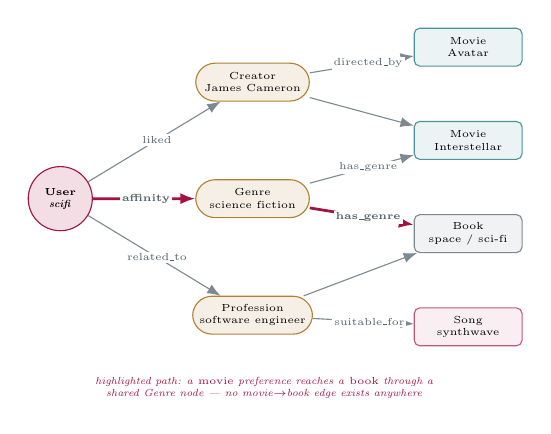
\begin{tikzpicture}[
  scale=0.74, transform shape, font=\tiny,
  usr/.style={circle, draw=amritaMaroon, fill=amritaMaroon!14, minimum size=11mm, align=center, font=\tiny\bfseries},
  ent/.style={rounded corners=7pt, draw=amritaAmber!80, fill=amritaAmber!10, align=center,
              minimum height=6.5mm, minimum width=1.95cm, font=\tiny},
  mv/.style={rounded corners=2pt, draw=amritaTeal!75, fill=amritaTeal!8, align=center,
              minimum height=6.5mm, minimum width=1.85cm, font=\tiny},
  bk/.style={rounded corners=2pt, draw=amritaSlate!75, fill=amritaSlate!8, align=center,
              minimum height=6.5mm, minimum width=1.85cm, font=\tiny},
  sg/.style={rounded corners=2pt, draw=amritaMaroon!70, fill=amritaMaroon!7, align=center,
              minimum height=6.5mm, minimum width=1.85cm, font=\tiny},
  e/.style={-{Latex[length=1.7mm]}, draw=amritaSlate!75, line width=0.4pt},
  hot/.style={-{Latex[length=1.9mm]}, draw=amritaMaroon, line width=1.0pt},
  el/.style={font=\tiny, text=amritaSlate, inner sep=1pt, fill=white}
]
\node[usr] (u)  at (0,3.0) {User\\\tiny\emph{scifi}};
\node[ent] (cr) at (3.3,5.0) {Creator\\\tiny James Cameron};
\node[ent] (gn) at (3.3,3.0) {Genre\\\tiny science fiction};
\node[ent] (pf) at (3.3,1.0) {Profession\\\tiny software engineer};

\node[mv] (m1) at (7.0,5.6) {Movie\\\tiny Avatar};
\node[mv] (m2) at (7.0,4.0) {Movie\\\tiny Interstellar};
\node[bk] (b1) at (7.0,2.4) {Book\\\tiny space / sci-fi};
\node[sg] (s1) at (7.0,0.8) {Song\\\tiny synthwave};

\draw[e]   (u)  -- (cr) node[el, pos=0.52] {liked};
\draw[hot] (u)  -- (gn) node[el, pos=0.52] {\textbf{affinity}};
\draw[e]   (u)  -- (pf) node[el, pos=0.52] {related\_to};
\draw[e]   (cr) -- (m1) node[el, pos=0.56] {directed\_by};
\draw[e]   (cr) -- (m2);
\draw[e]   (gn) -- (m2) node[el, pos=0.56] {has\_genre};
\draw[hot] (gn) -- (b1) node[el, pos=0.56] {\textbf{has\_genre}};
\draw[e]   (pf) -- (b1);
\draw[e]   (pf) -- (s1) node[el, pos=0.56] {suitable\_for};

\node[align=center, font=\tiny\itshape, text=amritaMaroon] at (3.5,-0.25)
  {highlighted path: a \emph{movie} preference reaches a \emph{book} through a\\shared Genre node --- no movie$\rightarrow$book edge exists anywhere};
\end{tikzpicture}
\end{center}
\vspace{-1mm}
{\tiny \textbf{Now:} in-memory \texttt{CatalogKnowledgeGraph} (pandas-backed, no external service, reranker contract already stable).
\textbf{Next:} the same contract re-hosted on Neo4j for multi-hop Cypher traversal and path-based explanations.}
\end{columns}
\end{frame}

% ---------------------------------------------------------------------
\begin{frame}{2. Evaluation -- Measured Results and Benchmark Status}
\framesubtitle{Scenario-level metrics (measured) $\cdot$ LightGCN holdout protocol (in progress)}
\vspace{-1mm}
\begin{columns}[T]
\column{0.55\textwidth}
{\scriptsize \textbf{(a) Measured prototype evaluation}}\\
{\tiny \hspace{1mm} 5 scenarios $\times$ demo profiles, via \texttt{scripts/evaluate\_recommendation\_table.py}}
\vspace{-1mm}
\begin{table}
\centering
\tiny
\renewcommand{\arraystretch}{1.16}
\begin{tabular}{p{1.95cm} p{1.75cm} c c c}
\toprule
\textbf{Scenario} & \textbf{Profile} & \textbf{Person} & \textbf{Profile} & \textbf{Avg.} \\
 & & \textbf{Hit@5} & \textbf{Align@5} & \textbf{KG} \\
\midrule
Actor / director & \texttt{user\_scifi} & 5/5 & 5/5 & 0.467 \\
Singer / artist & \texttt{user\_music\_pop} & 5/5 & 5/5 & 0.667 \\
Profession-aware & \texttt{user\_books\_learning} & --- & 5/5 & 0.250 \\
Family-safe & \texttt{user\_family} & --- & 5/5 & 0.533 \\
Cross-media intent & \texttt{user\_scifi} & --- & 5/5 & 0.400 \\
\midrule
\textbf{Aggregate} & & \textbf{1.00} & \textbf{1.00} & \textbf{0.463} \\
\bottomrule
\end{tabular}
\end{table}
\vspace{-2mm}
{\tiny Average profile alignment \textbf{0.803}; DomainCoverage@10 \textbf{0.60} --- 3 of 5 scenarios
returned more than one media type in the top-10.
Representative top-1 hits: \emph{Avatar} (James Cameron), \emph{Lover (Remix)} (Taylor Swift),
\emph{Minions} (family animation), \emph{Interstellar} (space adventure).}

\column{0.43\textwidth}
{\scriptsize \textbf{(b) LightGCN benchmark --- Amazon Reviews 2023}}
\vspace{-1mm}
\begin{table}
\centering
\tiny
\renewcommand{\arraystretch}{1.22}
\begin{tabular}{p{1.65cm} c c c}
\toprule
\textbf{Category} & \textbf{R@20} & \textbf{N@20} & \textbf{Status} \\
\midrule
Movies\_and\_TV & \mvRecall & \mvNDCG & trained \\
Books & --- & --- & \sWIP \\
CDs\_and\_Vinyl & --- & --- & \sWIP \\
\midrule
Popularity & --- & --- & control \\
\bottomrule
\end{tabular}
\end{table}
\vspace{-2mm}
{\tiny \textbf{Protocol.} Ratings $\geq 4$ binarised to implicit positives; iterative 10-core on
users and items; leave-last-out holdout per user; 200k-user sample; 60 epochs on a Kaggle T4;
ranked against a most-popular control. Amazon is $\sim$0.04\% dense, so R@20 in the
\textbf{0.03--0.08} band is the published operating range --- the claim under test is
\emph{LightGCN $>$ popularity on every metric}, not a large absolute value.}
\vspace{1.5mm}

{\scriptsize \textbf{(c) Engineering quality gate}}
\begin{itemize}\tiny
  \item \textbf{55 / 55} tests green in \textbf{7.81 s} --- preprocessing (27), embeddings (12), LightGCN (10), API (3), KG (3).
  \item Catalog rebuild is idempotent and hash-cached; the embedding rebuild skips unchanged rows.
\end{itemize}
\end{columns}
\vspace{-1mm}
{\tiny \textcolor{amritaSlate}{Books and CDs\_and\_Vinyl reuse the identical pipeline and notebook --- only the
\texttt{CATEGORY} constant changes --- and are scheduled ahead of Review 2.}}
\end{frame}

% =====================================================================
% SECTION 3 -- TECHNICAL KNOWLEDGE (Rubric: 5 Marks)
% =====================================================================
\section{Technical Knowledge}

\begin{frame}{3. Technical Knowledge \& Engineering Decisions}
\framesubtitle{Rubric: Software Architecture, Implementation, Integration \& Tech Stack (5 Marks)}
\vspace{-1mm}
\begin{columns}[T]
\column{0.49\textwidth}
{\scriptsize \textbf{Architectural \& design patterns}}
\begin{itemize}\tiny
  \item \textbf{Layered architecture} --- retrieval, storage, personalization and presentation are separately testable; the LightGCN artifact crosses a \emph{file} boundary, not a code boundary.
  \item \textbf{Repository pattern} --- \texttt{MySQLStore} is the single SQL surface; no query text lives in a route handler.
  \item \textbf{Dependency injection} --- FastAPI \texttt{Depends} resolves recommender / store / EMA singletons, so tests inject fakes without patching globals.
  \item \textbf{Lifespan singletons} --- heavy objects (SBERT model, Qdrant client) initialise once per worker. This is what fixed the \texttt{qdrant\_storage already locked} crash caused by \texttt{-{}-reload}'s multi-process spawn.
  \item \textbf{Strategy} --- every scoring head is an interchangeable reranker behind one contract; adding a head does not touch the pipeline.
  \item \textbf{Mapper} $\phi_d$ --- a new domain needs only a mapper; embedding, ANN, KG, API and UI stay untouched.
\end{itemize}
\vspace{0.5mm}
{\scriptsize \textbf{Data integrity \& concurrency}}
\begin{itemize}\tiny
  \item FK \texttt{user\_interactions.entity\_id} $\rightarrow$ \texttt{content\_entities.global\_id}, enforced in the schema \emph{and} pre-validated so the API returns 400, not 500.
  \item Idempotent \texttt{ON DUPLICATE KEY UPDATE} upserts --- re-running the loader is always safe.
  \item Composite index \texttt{(user\_id, timestamp)} serves the per-user history read on the hot path.
  \item Global vs. source IDs prevent primary-key collisions across the three datasets.
\end{itemize}

\column{0.49\textwidth}
{\scriptsize \textbf{Trade-offs we can defend}}
\begin{itemize}\tiny
  \item \textbf{Qdrant over FAISS} --- payload filtering by \texttt{content\_type} happens \emph{inside} the ANN search; FAISS required a second lookup and a post-filter.
  \item \textbf{BPR over MSE / BCE} --- feedback is implicit and positive-only, so there is no reliable negative label; ranking order is what we actually serve.
  \item \textbf{EMA over online gradient updates} --- one vector write per event instead of a parameter update; session drift is handled without touching item vectors.
  \item \textbf{In-memory KG over Neo4j (for now)} --- same scoring contract, zero extra service to deploy; migration is a swap, not a rewrite.
  \item \textbf{One 384-d space} --- items, queries and user vectors are all \texttt{all-MiniLM-L6-v2} outputs, so cosine applies directly with no projection layer.
  \item \textbf{GPU decoupling} --- training runs on a Kaggle T4; the served API is CPU-only and simply loads a small \texttt{.npz}.
\end{itemize}
\vspace{0.5mm}
{\scriptsize \textbf{Error handling, logging \& testing}}
\begin{itemize}\tiny
  \item Exception taxonomy mapped to HTTP: \texttt{ValueError}$\rightarrow$400; \texttt{FileNotFoundError} / \texttt{ImportError} / \texttt{RuntimeError}$\rightarrow$503, each with an actionable message.
  \item Graceful degradation --- a missing LightGCN artifact or EMA store disables that head only; the other four still rank.
  \item \textbf{55} pytest cases over 5 suites; Uvicorn access / error logs captured; \texttt{oxlint} on the frontend.
  \item \sPLN\ P95 latency benchmarking and load testing before Review 2.
\end{itemize}
\end{columns}
\end{frame}

% =====================================================================
% SECTION 4 -- TECHNICAL ENRICHMENT
% =====================================================================
\section{Technical Enrichment}

\begin{frame}{4. Technical Enrichment Activity Choices}
\framesubtitle{Professional Online Certification Details (Individual Mandatory: 10--20 Hours)}
    \begin{itemize}
        \item \textbf{Individual MOOC / Online Certification Selection:}
    \end{itemize}
    \vspace{-0.1cm}
    \begin{table}
        \centering
        \footnotesize
        \renewcommand{\arraystretch}{1.15}
        \begin{tabular}{|c|p{2.8cm}|p{4.4cm}|p{2.3cm}|c|}
            \hline
            \textbf{S.No} & \textbf{Student Name} & \textbf{Chosen MOOC / Course Title} & \textbf{Platform} & \textbf{Hours} \\
            \hline
            1 & Sanjay A. K. & Recommender Systems: Evaluation and Metrics & Coursera (U. Minnesota) & 15 Hrs \\
            \hline
            2 & Eswara Raj M. & Nearest Neighbor Collaborative Filtering & Coursera (U. Minnesota) & 14 Hrs \\
            \hline
            3 & Aditya Vijay & Databases and SQL for Data Science with Python & Coursera (IBM) & 20 Hrs \\
            \hline
            4 & Himaneesh Reddy J. & Recommendation Systems on Google Cloud & Google Cloud Skills Boost & 16 Hrs \\
            \hline
        \end{tabular}
    \end{table}
    \vspace{0.15cm}
    \begin{itemize}
        \item {\scriptsize \textbf{Direct project relevance:} the evaluation course maps onto the Recall@K / NDCG@K
        protocol on Slide 7; neighbourhood CF is the classical baseline LightGCN is measured against;
        SQL and indexing back the MySQL interaction store; the GCP course covers the candidate-generation
        and reranking split mirrored in our own pipeline.}
        \item {\scriptsize \textbf{Requirement:} each student completes one approved 10--20 hour certification from a
        recognised platform (Coursera, NPTEL, edX, Google Cloud) relevant to the project.
        Certificates to be submitted at Review 2.}
    \end{itemize}
\end{frame}

% =====================================================================
% REFERENCES
% =====================================================================
\section{References}
\begin{frame}[allowframebreaks]{References}
    \footnotesize
    \nocite{*}
    \bibliographystyle{IEEEtran}
    \bibliography{ref}
\end{frame}

% =====================================================================
% THANK YOU
% =====================================================================
\begin{frame}
    \centering
    {\Huge \textbf{\textcolor{amritaMaroon}{Thank You}}}\\[0.6cm]
    {\footnotesize \textcolor{amritaSlate}{Questions \& Panel Feedback}}
\end{frame}

\end{document}
